\documentclass[border=10pt,multi=tikzpicture]{standalone}
\usepackage{tikz}
\usetikzlibrary{shapes.callouts, shapes.symbols}

\begin{document}

% Page 1: Rectangle callout pointing lower-right
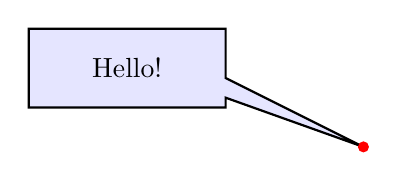
\begin{tikzpicture}
\node[rectangle callout, draw, thick, fill=blue!10,
      callout absolute pointer={(3,-1)},
      callout pointer width=0.25cm,
      minimum width=2.5cm, minimum height=1cm]
  {Hello!};
\fill[red] (3,-1) circle (2pt);
\end{tikzpicture}

% Page 2: Ellipse callout pointing upper-left
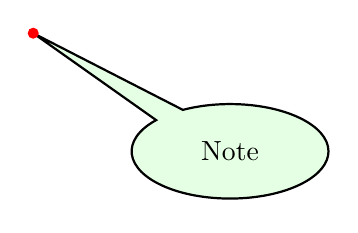
\begin{tikzpicture}
\node[ellipse callout, draw, thick, fill=green!10,
      callout absolute pointer={(-2.5,1.5)},
      callout pointer arc=20,
      minimum width=2.5cm, minimum height=1.2cm]
  {Note};
\fill[red] (-2.5,1.5) circle (2pt);
\end{tikzpicture}

% Page 3: Cloud shape (no callout)
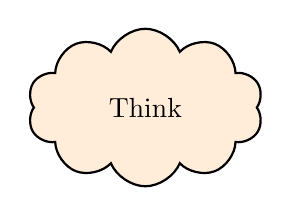
\begin{tikzpicture}
\node[cloud, draw, thick, fill=orange!15,
      cloud puffs=10, cloud puff arc=135,
      minimum width=3cm, minimum height=2cm]
  {Think};
\end{tikzpicture}

% Page 4: Cloud callout with thought bubbles
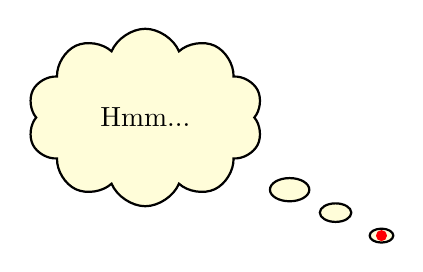
\begin{tikzpicture}
\node[cloud callout, draw, thick, fill=yellow!15,
      cloud puffs=10, cloud puff arc=135,
      callout absolute pointer={(3,-1.5)},
      callout pointer segments=3,
      minimum width=3cm, minimum height=2cm]
  {Hmm...};
\fill[red] (3,-1.5) circle (2pt);
\end{tikzpicture}

% Page 5: Rectangle callout pointing left
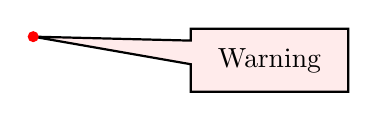
\begin{tikzpicture}
\node[rectangle callout, draw, thick, fill=red!8,
      callout absolute pointer={(-3,0.3)},
      callout pointer width=0.3cm,
      minimum width=2cm, minimum height=0.8cm]
  at (0,0) {Warning};
\fill[red] (-3,0.3) circle (2pt);
\end{tikzpicture}

\end{document}
